\subsection{Pastry/Tapestry}
\label{chap:evaluation_pastry}

\subsubsection*{Aufbau und Struktur}
Pastry \cite{Rowstron2001} und Tapestry \cite{Zhao2001Tapestry,Zhao2004Tapestry} sind sich sehr ähnlich, da beide auf Plaxtons Arbeit \cite{Plaxton1997Accessing} aufbauen. Auf Unterschiede wird explizit hingewiesen.

Pastry besitzt ebenfalls einen l-bit wertigen Schlüsselraum, dabei werden Schlüssel als Zahlen zur Basis $2^b$ dargestellt\footnote{l meist 128; b meist 4}, wobei die Wahl von $b$ einen Einfluss auf das Routing hat. Ein Datum ist dem Knoten zugewiesen, dessen ID den kleinesten Abstand zum Schlüsselwert des Datums hat.\\
\Fref{fig:pastry_key_space} zeigt dies beispielhaft für die gleichen sechs Knoten und fünf Datensätzen wie in \Fref[plain]{fig:chord_key_space}. Im Unterschied zu Chord ist jedoch Knoten $N14$ für $K16$ und Knoten $N54$ für $K55$ zuständig.

Tapestry erzeugt automatische Redundanz, da dessen Algorithmus die Daten automatisch auf mehrere Knoten verteilt.

\begin{figure}[htbp]
\centering
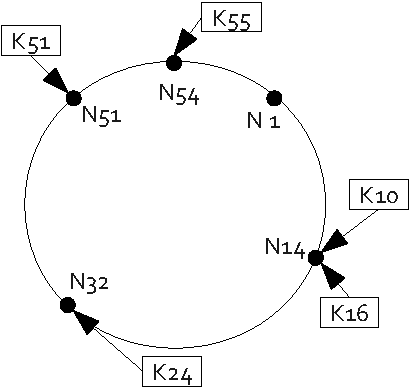
\includegraphics{grafics/pastry_key_space.pdf}
\caption{Schlüsselraum für Pastry mit sechs Knoten ($Nx$) und fünf Daten ($Kx$).}
\label{fig:pastry_key_space}
\end{figure}

\subsubsection*{Routing}
Jeder Knoten verwaltet neben den ihm zugeteilten Daten drei Strukturen die dem Routing dienen. Diese sind das \emph{leaf set} mit Einträgen zu Knoten die im Schlüsselraum benachbart sind, das \emph{neighborhood set} mit Einträgen zu Knoten die aus Netzwerksicht nahe liegen und die Routingtabelle selbst.

\begin{figure}[htbp]
\centering
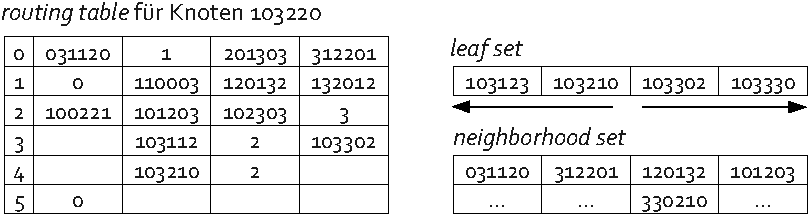
\includegraphics{grafics/pastry_routing_table.pdf}
\caption{Routing table, leaf set und neighborhood set bei Pastry}
\label{fig:pastry_routing_table}
\end{figure}

Die Routingtabelle besteht aus $\frac{l}{b}$ Reihen mit je $2^b -1$ Einträgen. \Fref{fig:pastry_routing_table} zeigt dies beispielhaft für Knoten $103220$ mit $l=12, b=2$ (nach \cite{Goetz2005}). Einträge in Zeile $i$ haben einen Präfix der Länge $i$ mit dem Knoten $103220$ gemein. Die Übereinstimmungen sind in der Abbildung fett hervorgehoben. Ist kein passender Knoten bekannt, wird das entsprechende Feld nicht ausgefüllt. Damit hat die Routingtabelle Ähnlichkeiten zur Fingertabelle bei Chord. Ein Knoten hat ungenaues Wissen über entfernte Knoten. Der Detailgrad an Routinginformationen erhöht sich pro Zeile in der Routingtabelle. Wenn im System nur sehr wenig Knoten vorhanden sind, dann sind die letzten Reihen der Routingtabelle ebenfalls nur spärlich belegt. Im Durchschnitt sind bei $n$ Knoten im System nur $log_{2^b} n$ Einträge belegt.\\
Bei der Belegung der Routingtabelle werden bei gleichem Präfix diejenigen Knoten gewählt, die aus Netzwerksicht näher sind.

Das leaf set enthält die $l$ numerisch nahen Knoten, $\frac{l}{2}$ davon sind kleiner und $\frac{l}{2}$ größer als der aktuelle Knoten. Neben Informationen zu Routingentscheidungen wird es zur Reparatur genutzt, sollten nahe gelegene Knoten ausfallen.

Das eigentlich Routing unterscheidet zwei Fälle: Zuerst prüft der Knoten ob der Schlüssel $k$ im Bereich seines leaf set ist. Ist dies der Fall, wird die Nachricht an den entsprechenden Knoten gesendet. Ist dieser Knoten für den Schlüssel zuständig, endet das Routing. Fällt $k$ nicht in den Bereich des leaf set, wird die Nachricht via Routingtabelle an einen entfernteren Knoten gesendet. Hierzu wird ein Eintrag gewählt, der eine größere beziehungsweise die größte Prefixübereinstimmung mit $k$ hat. Existiert kein solcher Eintrag, wird die Nachricht an den numerisch nächsten Knoten (zu $k$) mit gleicher Präfixübereinstimmung geschickt.\\
Da Nachrichten immer an Knoten mit einer größeren Übereinstimmung oder an nähere Knoten mit gleicher Präfixübereinstimmung gesendet werden, können keine Zyklen auftreten.

Dadurch verringert sich die Anzahl der Knoten mit längeren Präfixübereinstimmungen in jedem Schritt um mindestens den Faktor $2^b$. Somit hat das Routing eine Komplexität von $O(log_{2^b} N)$.

Das Routing von Tapestry ist sehr ähnlich zu dem hier vorgestellten Routing, allerdings nutzt Tapestry ein suffix-basiertes System. Ebenso speichert Tapestry in einem Eintrag der Routingtabelle mehrer mögliche Peers. So kann bei einem Ausfall schneller ein Ersatz gefunden werden.

\subsubsection*{Nachbarschaft}
Das neighborhood set (siehe \Fref{fig:pastry_routing_table}) enthält $|m|$ Knoten die aus Netzwerksicht nahe sind. Obwohl es im Routing keine Rolle spielt kann es dazu genutzt werden in späteren Entscheidungen geeignete Knoten zu finden.\\
Da die Größe des leaf set ebenfalls wählbar ist, können hier ebenfalls vermehrt nahe Knoten platziert werden.

\subsubsection*{Eintritt und Austritt (Fehlerfall) von Knoten}
Einem neuen Knoten $n$ wird von Applikationsseite ein frei wählbarer Schlüssel gegeben. Meist berechnet sich dieser Schlüssel anhand dem Hashwert der IP oder seines öffentlichen Namens. Weiterhin geht das System davon aus, dass $n$ aus einer Liste bekannter Knoten denjenigen Knoten $x$ wählen kann, der aus Netzwerksicht nahe ist. Von diesem Knoten kann das neighborhood set kopiert werden. Zum Aufbau der Routingtabelle und des leaf set lässt $n$ via $x$ eine \emph{JOIN}-Nachricht an einen numerisch nahen Schlüssel zu $n$ routen. Diese Nachricht gelangt schließlich zu Knoten $c$, von dem das leaf set kopiert werden kann, da $c$ und $n$ sich nahe sind. Alle Knoten die diese \emph{JOIN}-Nachricht weiterleiten, senden ihre Routingtabelle an $n$. Für jeden Routinghop kopiert sich $n$ die entsprechende Zeile aus der Routingtabelle, da ausgehend von keiner Präfixübereinstimmung mit dem nahen Knoten $x$, jeder weitere Hop eine größere Präfixübereinstimmung bringt.\\
Im Gegensatz zur nachträglichen Aktualisierung bei Chord, wird nun die gesamte Routinginformation an alle bekannte Knoten gesendet. Der neue Knoten ist nun im Netzwerk bekannt und erreichbar.

Ausgefallene Knoten werden ebenfalls anhand von Timeouts beim Routing entdeckt. Da die Einträge des neighborhood set nicht im Routing involviert sind, müssen diese periodisch geprüft werden. Fehlerhafte Einträge in der Routingtabelle können über einen anderen Eintrag mit gleicher Präfixübereinstimmung kompensiert werden, müssen aber entfernt werden um ein stabiles und sicheres Routing zu gewährleisten. Hierzu können von benachbarten Einträgen Routinginformationen angefordert werden um die entstandene Lücke zu füllen. Ein fehlerhafter Eintrag im leaf set oder neighborhood set kann auf ähnliche Weise repariert werden: Hier werden Informationen von den anderen Einträgen im leaf set oder neighborhood set angefordert.

Der Austritt eines Knotens wird vom System wie ein Fehlerfall behandelt werden. Um die Datenintegrität zu gewährleisten und um unnötigen Nachrichtenversand im System zu vermeiden, sollte die Applikation den Austritt eines Knotens speziell behandeln.

